\documentclass[11pt,notes=hide,aspectratio=169,mathserif]{beamer}

% PACKAGES
\usepackage{graphics}
\usepackage{graphicx}  % \resizebox
\usepackage{url}
%\usepackage{natbib}
\usepackage{bibentry}
\usepackage{verbatim}
\usepackage{booktabs}
\usepackage{etoolbox}
\usepackage{datetime}
\usepackage{bm}
\usepackage{subcaption}
\usepackage{amsfonts}
\usepackage{amsmath}
\usepackage{amsthm}

% CUSTOM DEFINITIONS
\def\newblock{} % Get beamer to cooperate with BibTeX
\linespread{1.2}

% IDENTIFYING INFORMATION
\title[class]{ECON 340: Economics of the Family \\ TA Session 2}
\author[Vaidehi's class]{Vaidehi Parameswaran (Northwestern Economics)}
\date{\monthname[\the\month] \the\year}

% THEME OPTIONS
\usetheme{metropolis}
\definecolor{mycolor}{RGB}{48,7,144}
\setbeamercolor{frametitle}{bg=mycolor, fg=white}
\setbeamercolor{title separator}{fg=mycolor}
\setbeamercolor{progress bar}{fg=mycolor}
\beamertemplatenavigationsymbolsempty
\setbeamertemplate{footline}[frame number]{}
\setbeamertemplate{itemize item}{\small\raisebox{1pt}{\textcolor{mycolor}{$\blacktriangleright$}}}
\setbeamertemplate{itemize subitem}{\footnotesize\raisebox{1pt}{\textcolor{mycolor}{$\triangleright$}}}
\setbeamertemplate{itemize subsubitem}{\tiny\raisebox{1pt}{\textcolor{mycolor}{$\triangleright$}}}

% Clickable links
\usepackage{hyperref}
\hypersetup{
  colorlinks=true,
  linkcolor=mycolor,
  urlcolor=mycolor,
  citecolor=mycolor
}

% BACKUP SLIDE NUMBERING
\usepackage{appendixnumberbeamer}

% Show a bulleted mini-contents slide at each section
% Bulleted ToC using your triangle icons + color
\setbeamertemplate{section in toc}{%
  \leavevmode\llap{\textcolor{mycolor}{$\blacktriangleright$}\hspace{0.6ex}}%
  \inserttocsection\par}
\setbeamertemplate{subsection in toc}{%
  \leavevmode\llap{\textcolor{mycolor}{$\triangleright$}\hspace{1.1ex}}%
  \inserttocsubsection\par}

\AtBeginSection[]{
  \begin{frame}{Today}
    \tableofcontents[currentsection]
  \end{frame}
}

\begin{document}

%---------------------------------------------------------------------
\begin{frame}[plain]
\titlepage
\end{frame}
%---------------------------------------------------------------------

\section{The Economics of Dowry and Brideprice}

%---------------------------------------------------------------------
\begin{frame}{Prevalence of Marriage Payments}
\begin{itemize}
  \item Bride price—dates back to 3000 BCE in Egyptian, Mesopotamian, Hebrew, Aztec, and Inca civilizations.
  \item Dowry—dates back to Greco-Roman times.
  \begin{itemize}
    \item In contemporary times, it is most extensively documented in India.
  \end{itemize}
  \item Payments are often very large relative to income.
\end{itemize}
\end{frame}
%---------------------------------------------------------------------
%---------------------------------------------------------------------
\begin{frame}{Magnitude of Marriage Payments}
  \begin{figure}
  \centering
  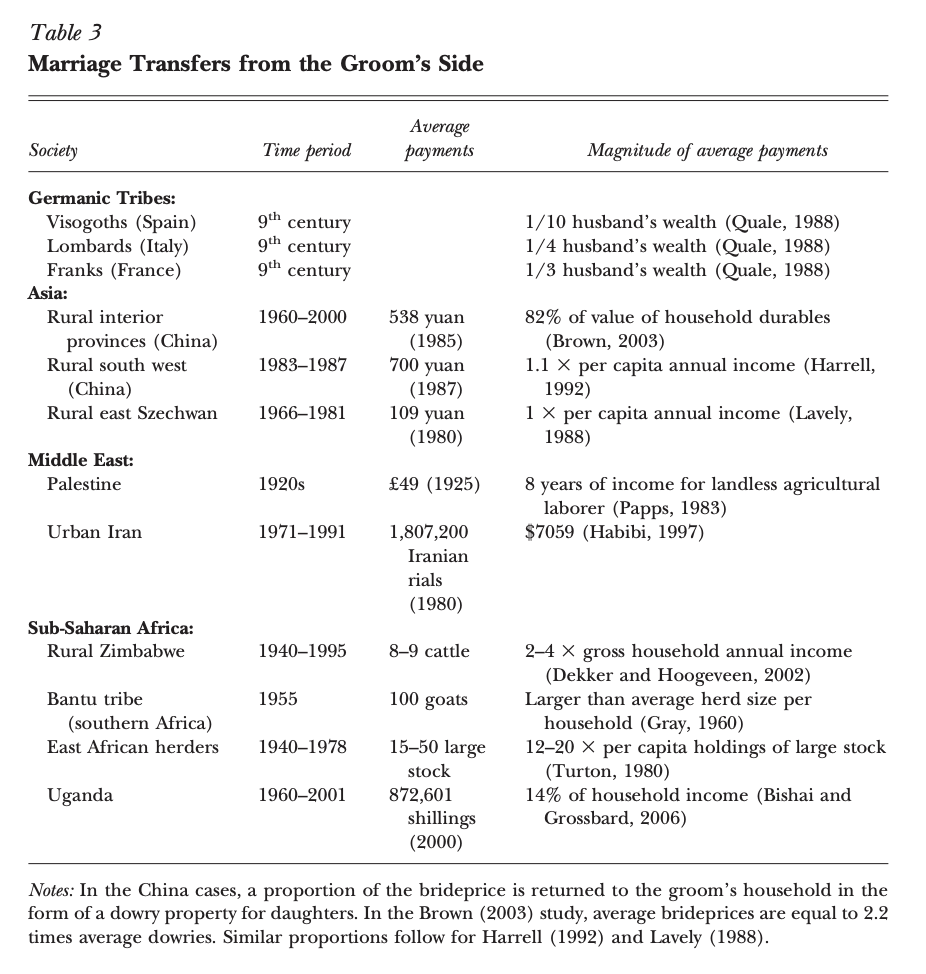
\includegraphics[width=0.5\linewidth]{inputs/magn2.png}
  \label{fig:marriage_payments}
  \end{figure}
\end{frame}
%---------------------------------------------------------------------

%---------------------------------------------------------------------
\begin{frame}{Magnitude of Marriage Payments}
  \begin{figure}
  \centering
  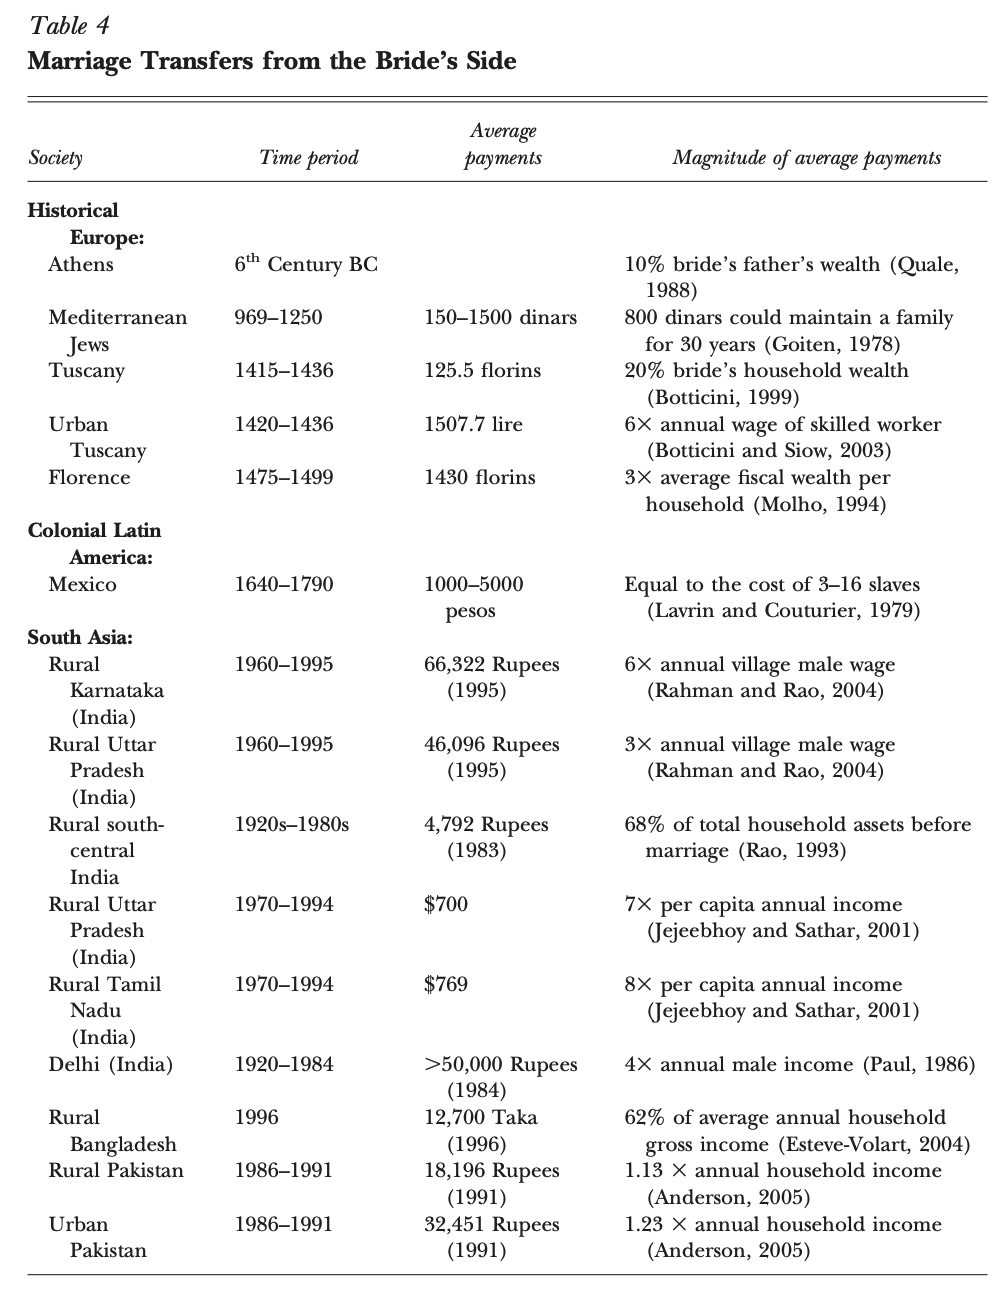
\includegraphics[width=0.5\linewidth]{inputs/magnitude.png}
  \label{fig:marriage_payments}
  \end{figure}
\end{frame}
%---------------------------------------------------------------------


\section{Bride Price and Female Education — Ashraf et al., 2020}

%---------------------------------------------------------------------
\begin{frame}{Overview}
\begin{itemize}
  \item Culture is important for economic development.
  \item Much more needs to be done to understand the role of traditional practices in development policy.
  \item This paper revisits well-studied school construction programs in Indonesia and Zambia.
  \item In particular, it aims to understand how bride price impacts the effects of these programs.
\end{itemize}
\end{frame}
%---------------------------------------------------------------------


%---------------------------------------------------------------------
\begin{frame}{Overview of the Model}
\begin{itemize}
  \item Imperfectly altruistic parents decide on investments in their children's education.
  \item After children become adults, there is a matching market for marriage and education is complementary in the marriage market.
  \item Bride price is the marital transfer to the bride that is appropriated by the bride’s parents.
  \item Thus, in equilibrium, the bride price is increasing in the education of the bride.
  \item Bride price provides an additional monetary incentive for parents to invest in their daughters’ education.
  \item When female education rates are low, a decline in the cost of schooling increases education more for girls from bride-price ethnic groups than for girls from non--bride-price ethnic groups.
\end{itemize}
\end{frame}
%---------------------------------------------------------------------

%---------------------------------------------------------------------
\begin{frame}{Bride Price Custom}
  \begin{figure}
    \centering
    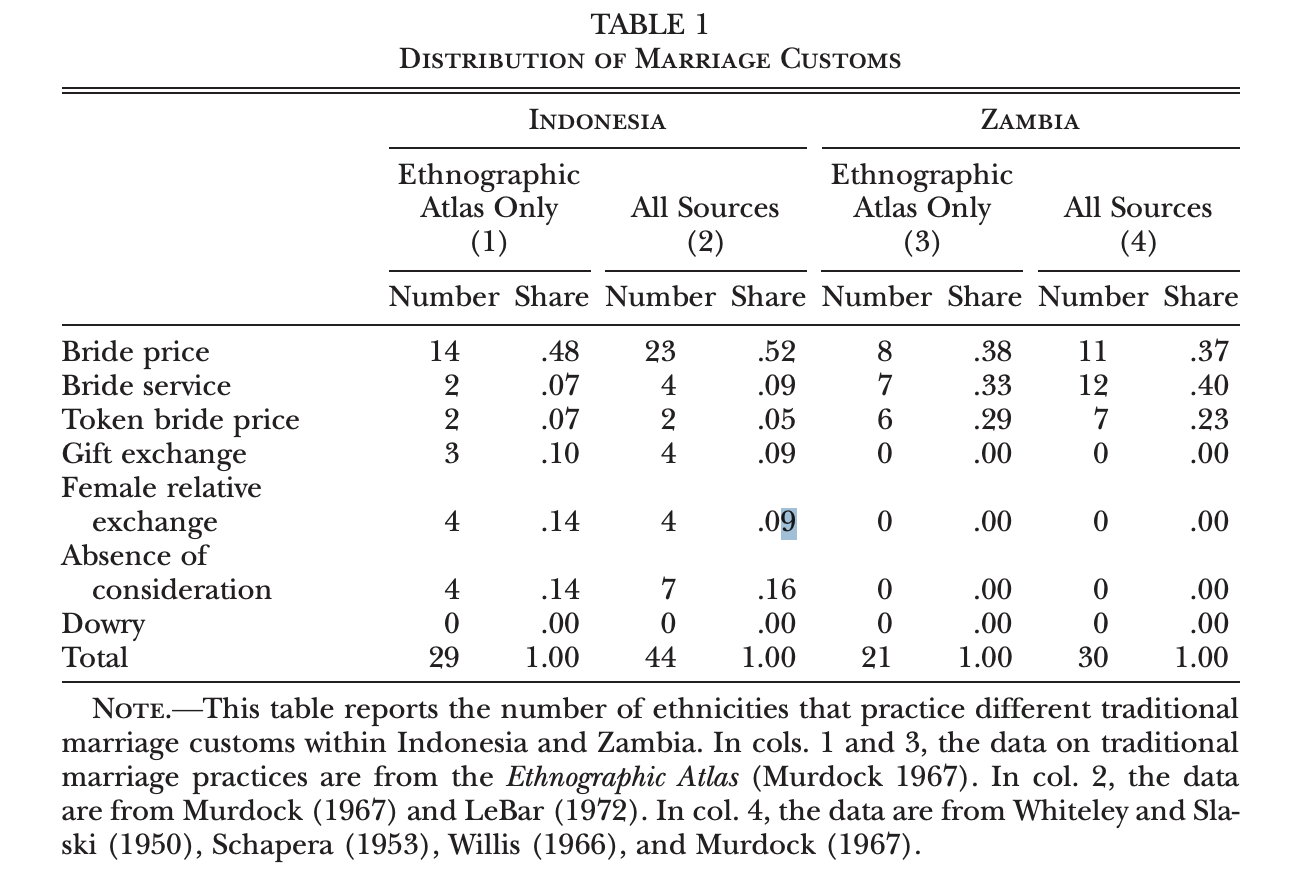
\includegraphics[width=0.8\linewidth]{inputs/bride_price_table.png}
    \label{fig:bride_price_table}
    \end{figure}
\end{frame}
%---------------------------------------------------------------------

%---------------------------------------------------------------------
\begin{frame}{Bride Price Custom}
  \begin{figure}
    \centering
    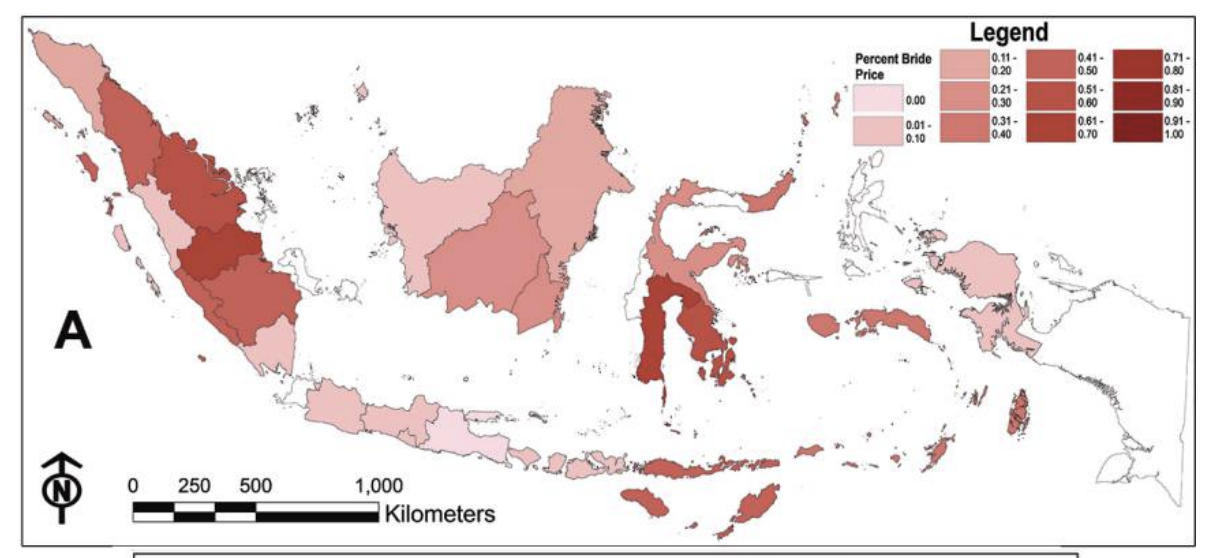
\includegraphics[width=0.6\linewidth]{inputs/bride_price_ind.png}
    \caption{Bride price in Indonesia}
    \label{fig:bride_price_ind}
    \end{figure}
\end{frame}
%---------------------------------------------------------------------

%---------------------------------------------------------------------
\begin{frame}{Bride Price Custom}
  \begin{figure}
    \centering
    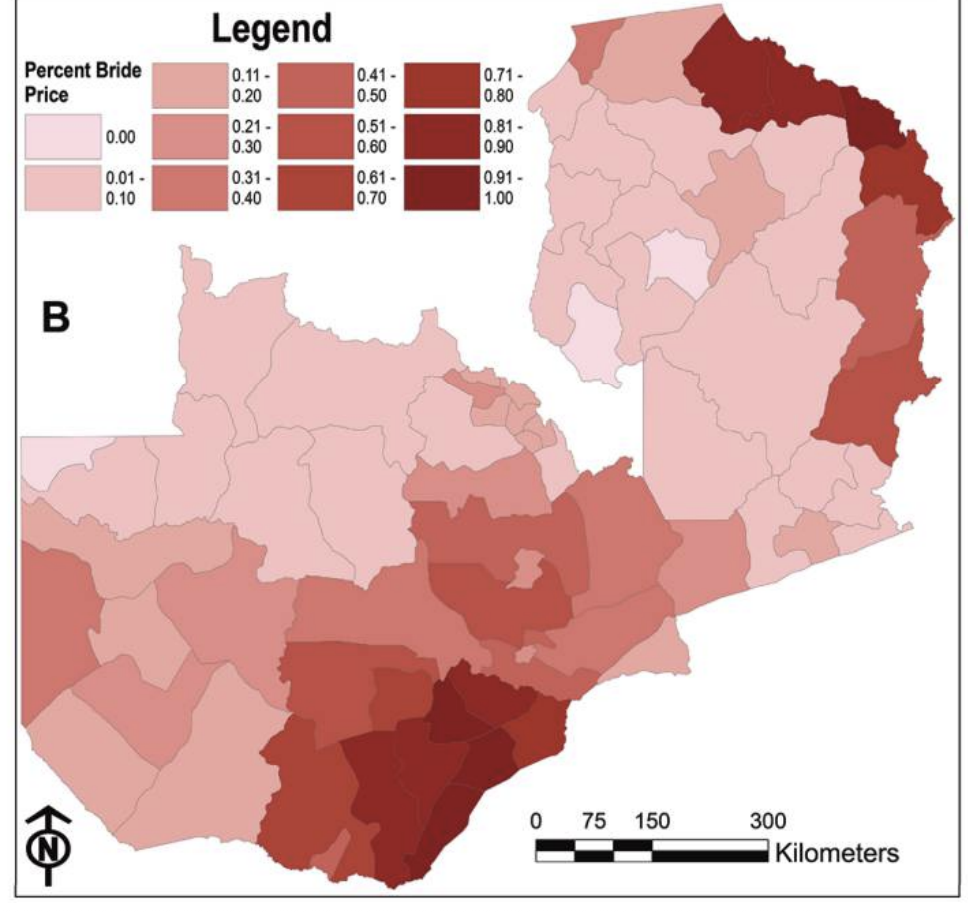
\includegraphics[width=0.5\linewidth]{inputs/bride_price_zam.png}
    \caption{Bride price in Zambia}
    \label{fig:bride_price_zam}
    \end{figure}
\end{frame}
%---------------------------------------------------------------------

%---------------------------------------------------------------------
\begin{frame}{Prediction 1: Is Matching Assortative by Education?}
  \begin{figure}
    \centering
    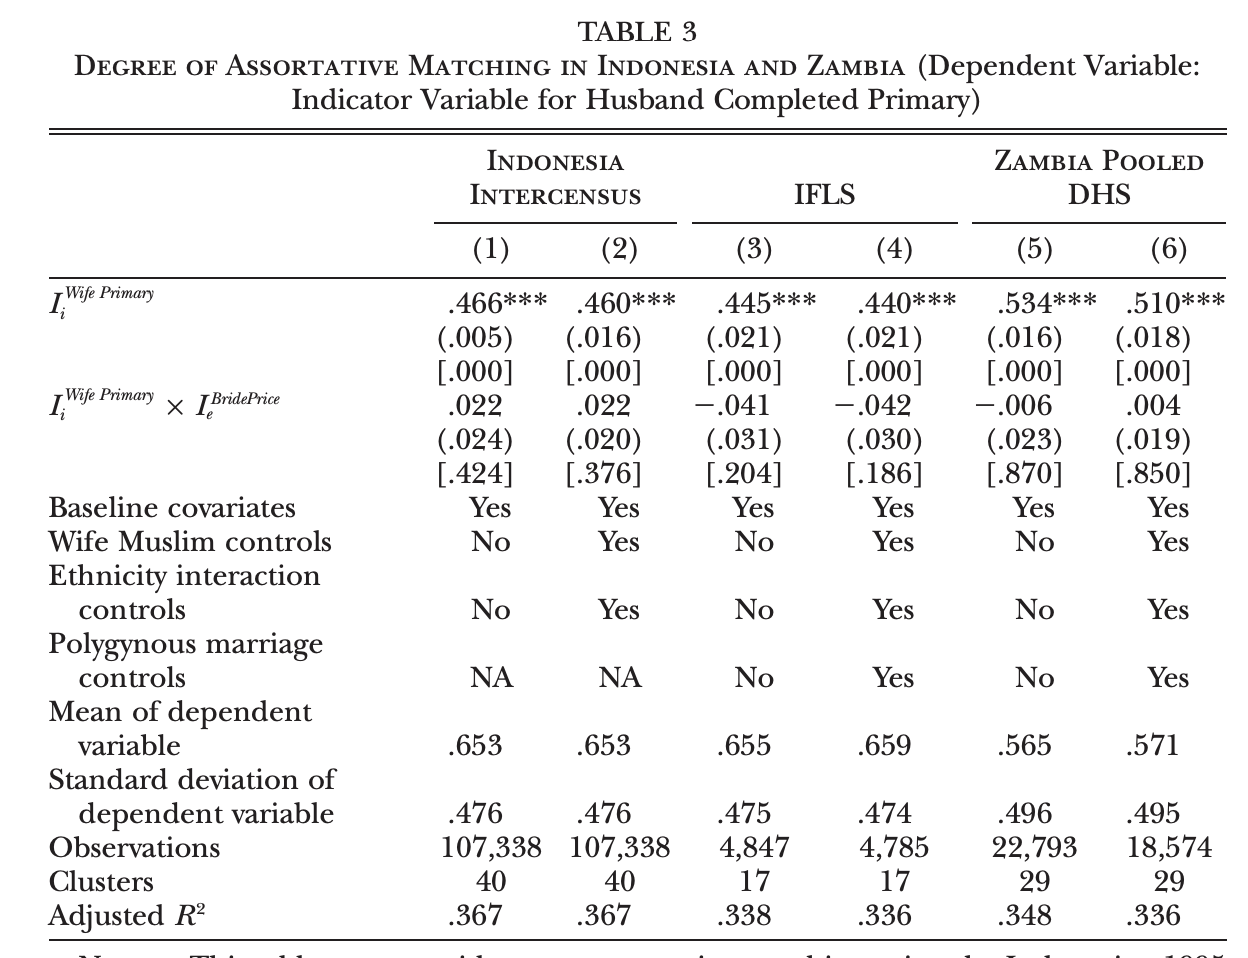
\includegraphics[width=0.6\linewidth]{inputs/pred1.png}
    \caption{Assortative Matching}
    \label{fig:pred1}
    \end{figure}
\end{frame}
%---------------------------------------------------------------------

%---------------------------------------------------------------------
\begin{frame}{Prediction 2: Do Bride Price Amounts Increase with the Bride’s Education?}
  \begin{figure}
    \centering
    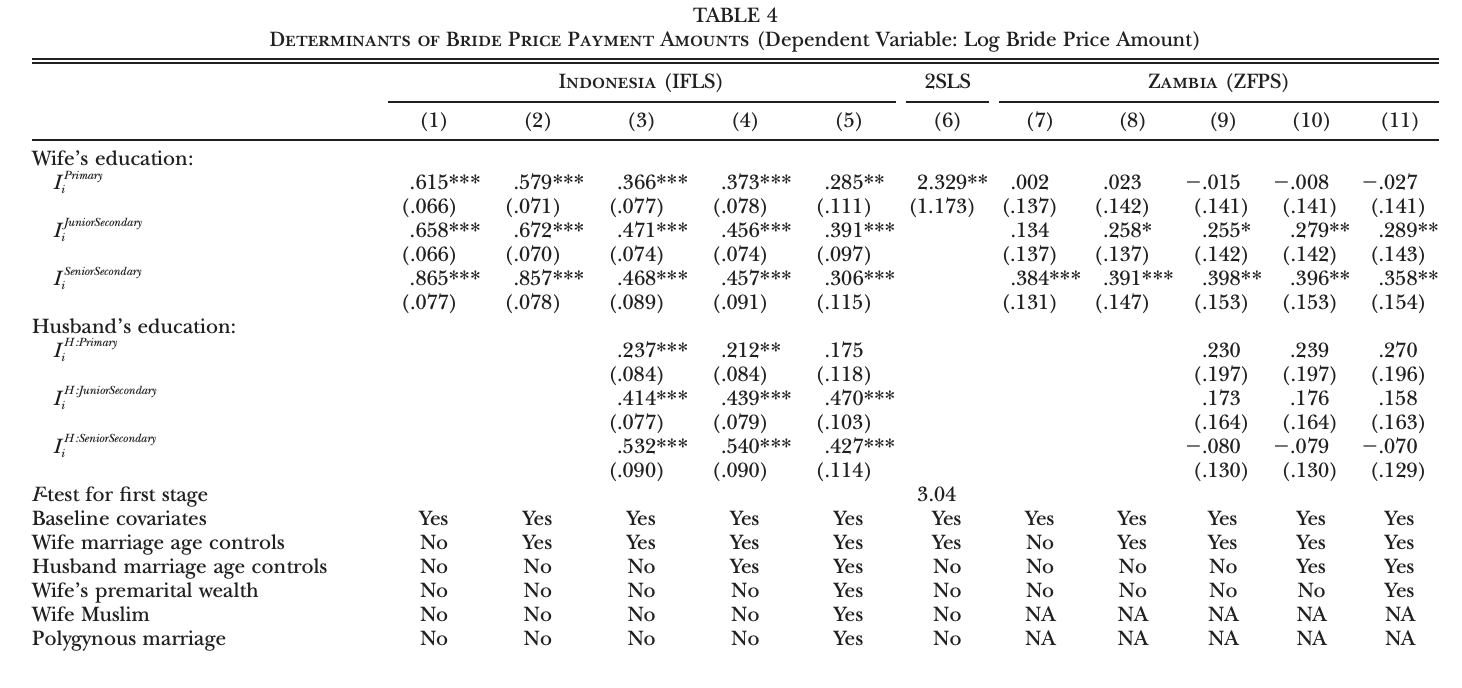
\includegraphics[width=0.9\linewidth]{inputs/pred2.png}
    \label{fig:pred2}
    \end{figure}
\end{frame}
%---------------------------------------------------------------------

%---------------------------------------------------------------------
\begin{frame}{Prediction 3: Do Bride-Price Groups Have Higher Rates of Female Education?}
  \begin{figure}
    \centering
    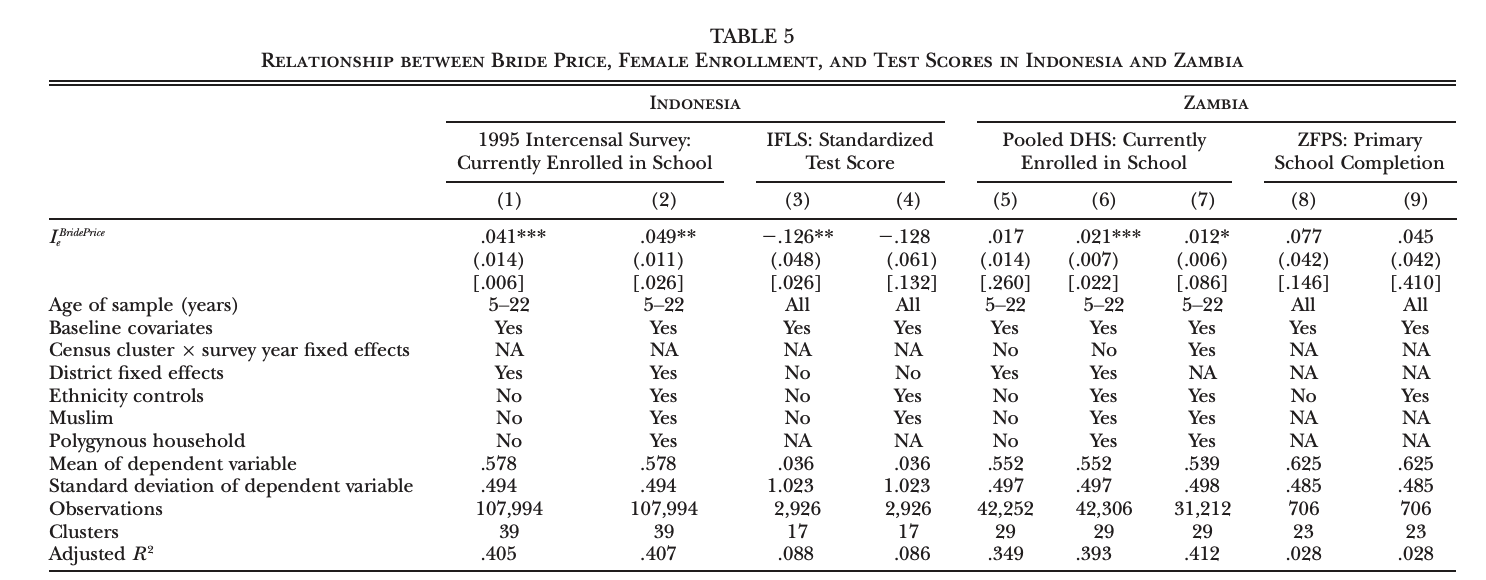
\includegraphics[width=1\linewidth]{inputs/pred3.png}
    \label{fig:pred3}
    \end{figure}
\end{frame}
%---------------------------------------------------------------------

%---------------------------------------------------------------------
\begin{frame}{Prediction 4: Differential Effects of Education Policies}
  \begin{figure}
    \centering
    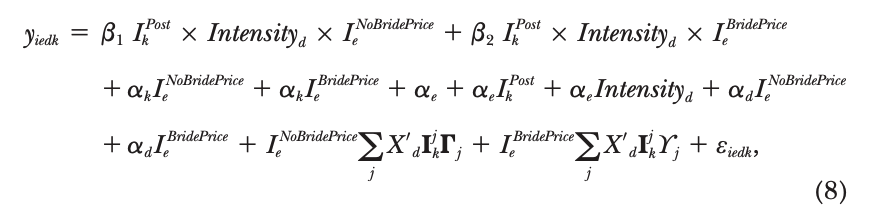
\includegraphics[width=1\linewidth]{inputs/eq.png}
    \label{fig:pred4_eq}
    \end{figure}
    \begin{itemize}
        \item A difference-in-differences setup (as in Duflo, 2001).
        \item Heterogeneity by the bride-price custom.
    \end{itemize}
\end{frame}
%---------------------------------------------------------------------

%---------------------------------------------------------------------
\begin{frame}{Prediction 4: Differential Effects of Education Policies}
  \begin{figure}
    \centering
    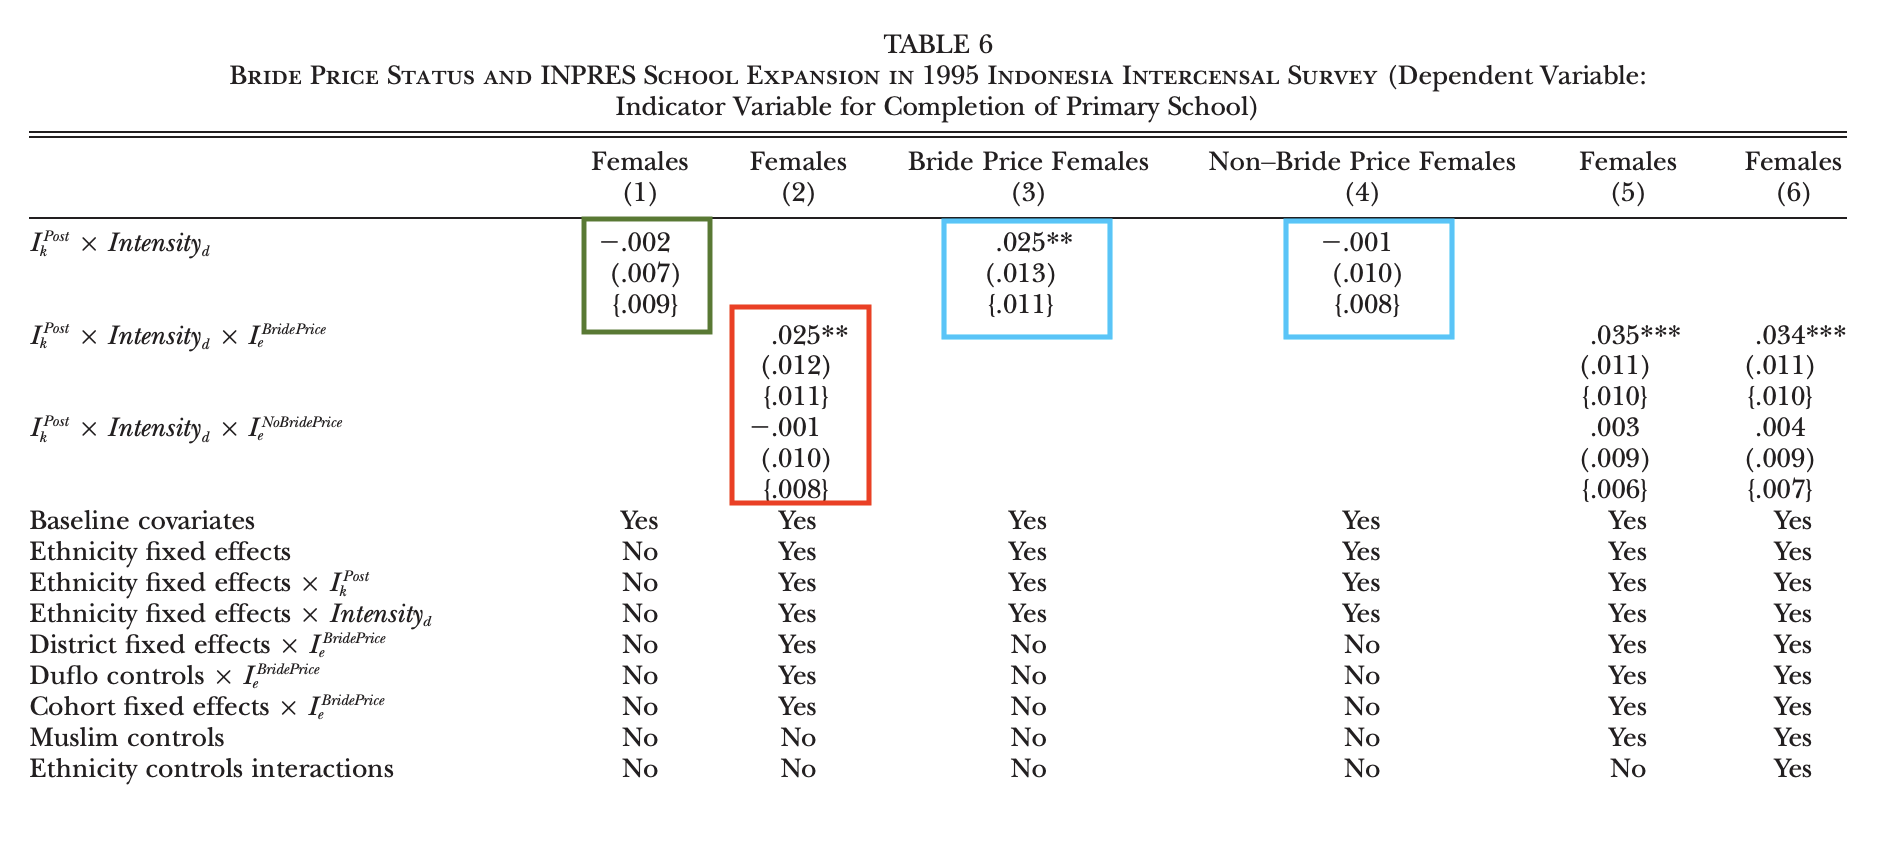
\includegraphics[width=1\linewidth]{inputs/pred4.png}
    \caption{Main Prediction}
    \label{fig:pred4}
    \end{figure}
\end{frame}
%---------------------------------------------------------------------


%---------------------------------------------------------------------
\begin{frame}{What the Authors Find}
  \begin{itemize}
    \item Girls belonging to bride-price ethnic groups are more likely to be educated.
    \item Bride-price ethnic groups are more responsive to policies aimed at increasing female education.
    \item In both Indonesia and Zambia:
    \begin{itemize}
        \item For bride-price ethnic groups, the increased supply of schools resulted in a significant increase in female education.
        \item For those without the bride-price custom, the program had no effect on female education.
    \end{itemize}
    \item In the context of educational policies, it is not immediately obvious that marriage customs would play a role.
    \item A lesson to be learned: culture matters for policy!
    \end{itemize}
\end{frame}
%---------------------------------------------------------------------


%---------------------------------------------------------------------
\begin{frame}
\begin{center}{\LARGE See you next time!}\end{center}
\end{frame}
%---------------------------------------------------------------------


% \beginbackup
% \appendix
% \input{sections/appendix.tex}
% \bibliographystyle{../bib/aeanobold}
% \nobibliography{../bib/bib.bib}
% \backupend

\end{document}
